\section{Introduction}
Neural networks (NNs) and decision trees (DTs) are both powerful classes of machine learning models with proven successes in academic and commercial applications. The two approaches, however, typically come with mutually exclusive benefits and limitations, as illustrated in Fig.~\ref{fig:pros_and_cons}.

\begin{figure*}[ht]
	\center
	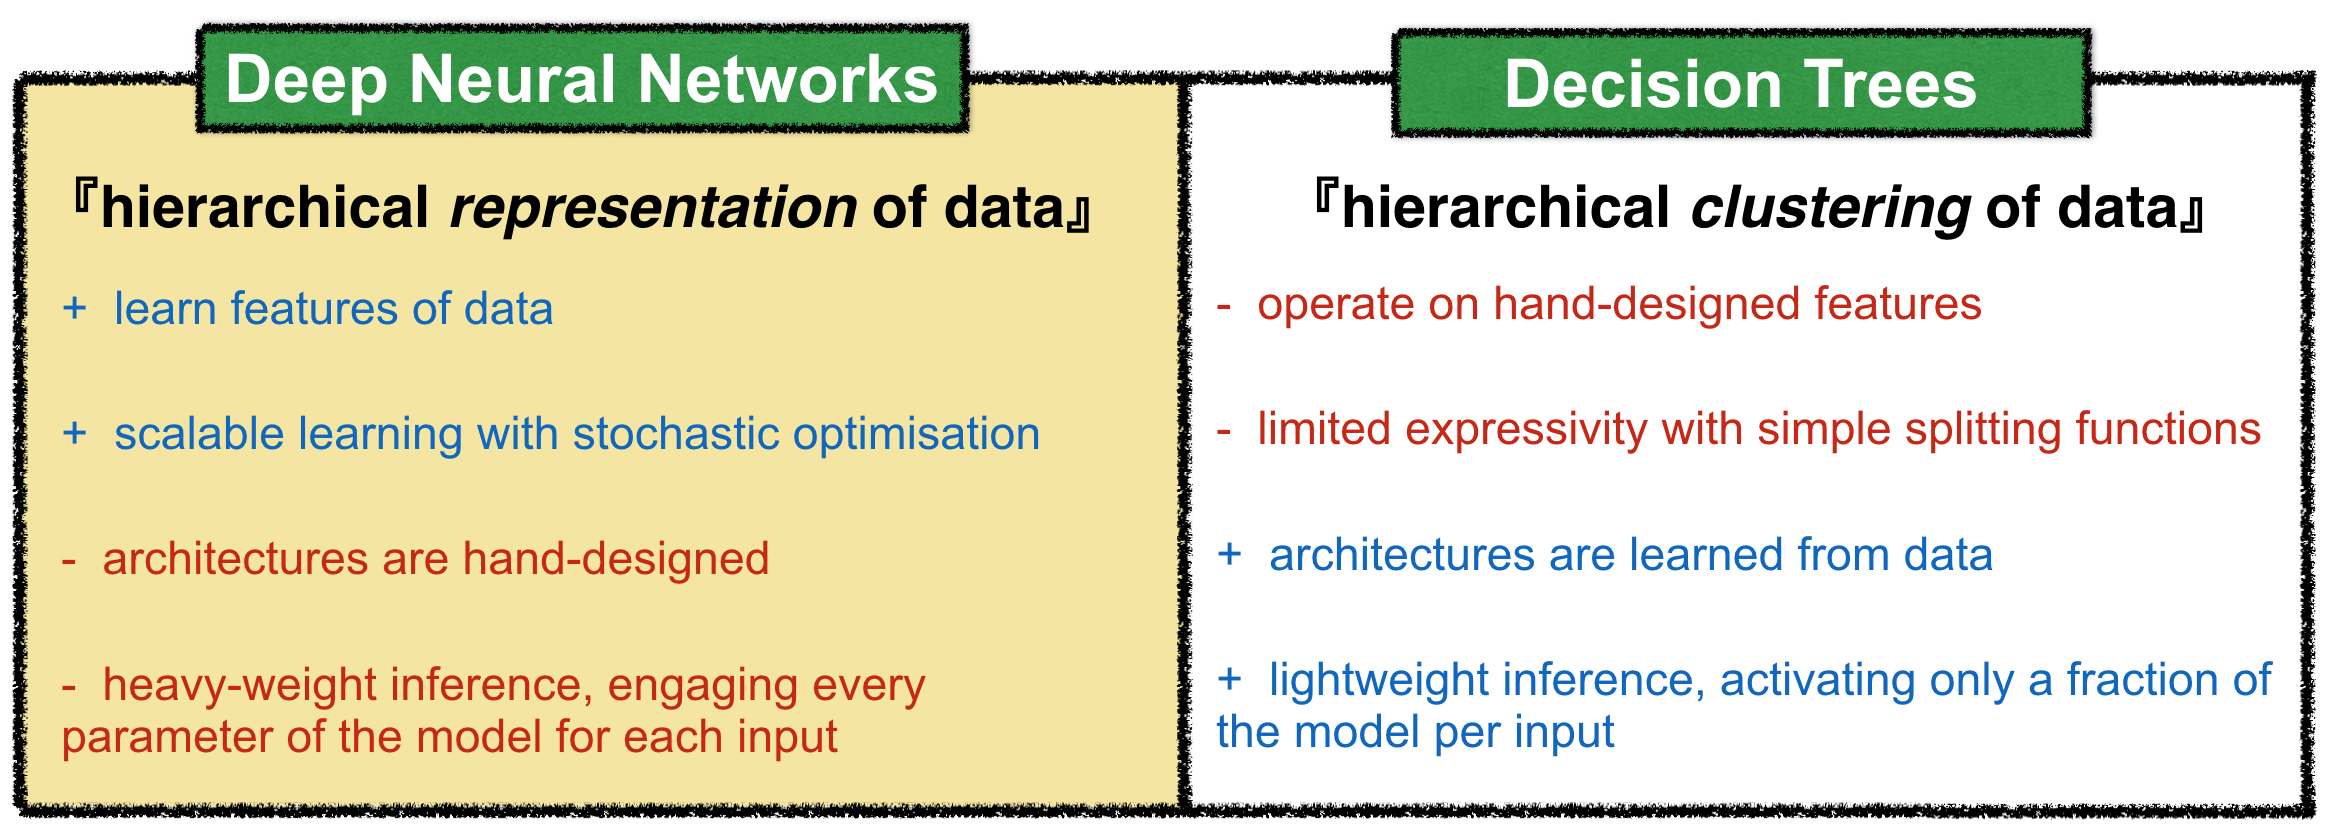
\includegraphics[width=0.85\linewidth]{chapter_7/figures/pros_and_cons.png}
	\caption{\small Comparison of two machine learning paradigms. }
	\label{fig:pros_and_cons}
\end{figure*}

%DNNs are characterised by learning hierarchical representation of data \cite{zeiler2014visualizing,bengio2013deep}. In the supervised learning setting, DNNs are capable of learning complex non-linear transformations to apply to input data, so a simple linear model can adequately perform the predictive task of interest.
NNs are characterised by learning hierarchical representations of data through the composition of nonlinear transformations \cite{zeiler2014visualizing,bengio2013deep}, % In classification, for example, the final representations of different classes are trained to become linearly separable.
which has alleviated the need for feature engineering, in contrast to many other machine learning models. In addition, NNs are trained with stochastic optimisers, such as stochastic gradient descent (SGD), allowing training to scale to large datasets. Consequently, with modern hardware, we can train NNs of many layers on large datasets, solving numerous problems ranging from object detection to speech recognition with unprecedented accuracy \cite{lecun2015deep}. However, their architectures typically need to be designed by hand and fixed per task or dataset, requiring domain expertise \cite{zoph2016neural}. Inference can also be heavy-weight for large models, as each sample engages every part of the network, i.e., increasing capacity causes a proportional increase in computation \cite{bengio2013estimating}. 

%The last few years have seen an incredible rise in the use of deep neural networks (DNNs), typically with large amounts of data, to solve tasks ranging from object detection to speech recognition \cite{lecun2015deep}. DNNs embody the ethos of deep learning, that is based on learning hierarchical representations of data \cite{bengio2013deep}. A notable example is that of convolutional neural networks (CNNs) trained for object recognition, learning oriented edges at the bottom of the network, textures in the middle, and object parts at the top \cite{zeiler2014visualizing}. However, most NN architectures are specifically hand-designed for one task or dataset, requiring domain expertise.

Alternatively, DTs are characterised by learning hierarchical clusters of data \cite{criminisi2013decision}. A DT learns how to split the input space, so that in each subset, linear models suffice to explain the data. In contrast to standard NNs, the architectures of DTs are optimised based on training data, and are particularly advantageous in data-scarce scenarios. DTs also enjoy lightweight inference as only a single root-to-leaf path on the tree is used for each input sample. However, successful applications of DTs often require hand-engineered features of data. We can ascribe the limited expressivity of single DTs to the common use of simplistic routing functions, such as splitting on axis-aligned features. The loss function for optimising hard partitioning is non-differentiable, which hinders the use of gradient descent-based optimization and thus complex splitting functions. Current techniques for increasing capacity include ensemble methods such as random forests (RFs) \cite{breiman2001random} and gradient-boosted trees (GBTs) \cite{friedman2001greedy}, which are known to achieve state-of-the-art performance in various tasks, including medical applications and financial forecasting \cite{sandulescu2016predicting,kaggle2017,le2016lifted,volkovs2017content}.

The goal of this work is to combine NNs and DTs to gain the complementary benefits of both approaches. To this end, we propose \textit{adaptive neural trees} (ANTs), which generalise previous work that attempted the similar unification \cite{suarez1999globally,irsoy2012soft,laptev2014convolutional,rota2014neural,kontschieder2015deep,frosst2017distilling,xiao2017ndt} and address their limitations (see Tab. \ref{tab:comparison}). 
%While previous works based on DTs have required partitioning the data at every level of the model, ANTs allow for extended sequences of nonlinear transformations in-between---the key to the success of NNs.
ANTs represent routing decisions and root-to-leaf computational paths within the tree structures as NNs, which lets them benefit from hierarchical representation learning, rather than being restricted to partitioning the raw data space. On the other hand, unlike the fully distributed representation of standard NN models, the tree topology of ANTs acts as a strong structural prior that enforces sparse structures by which features are shared and separated in a hierarchical fashion. In addition, we propose a backpropagation-based training algorithm to grow ANTs based on a series of decisions between making the ANT deeper---the central NN paradigm---or partitioning the data---the central DT paradigm (see Fig.~\ref{fig:hierarchy} (Right)). This allows the architectures of ANTs to adapt to the data available. By our design, ANTs inherit the following desirable properties from both DTs and NNs:

%The goal of this work is to combine NNs and DTs to gain the complementary benefits of both approaches. To this end, we propose \textit{adaptive neural trees} (ANTs), which consist of two key innovations: (1) a novel form of DTs, where computational paths and routing decisions are represented by NNs; (2) a backpropagation-based training algorithm which grows the architecture from simple modules. Furthermore, ANTs generalise previous work that attempted the same unification \cite{suarez1999globally,irsoy2012soft,laptev2014convolutional,rota2014neural,kontschieder2015deep,frosst2017distilling,xiao2017ndt} and address their limitations (see Fig. \ref{fig:hierarchy}(Right)). In particular, ANTs inherit the following desirable properties from both DTs and NNs:

% (RYu) During which each leaf node of the tree optimises the choice between "going deeper" and partioning the data until meeting some termination criteria. The proposed method generalises many previous works that attempted the same unification \cite{rota2014neural,kontschieder2015deep,ioannou2016decision,frosst2017distilling} and address their limitations (see Table. \ref{table:comparison}).
\begin{itemize}
	\item \textbf{Representation learning}: as each root-to-leaf path in an ANT is an NN, features can be learned end-to-end with gradient-based optimisation. Combined with the tree structure, an ANT can learn such features which are hierarchically shared and separated. The training algorithm is also amenable to SGD.
	
	\item \textbf{Architecture learning}: by progressively growing ANTs, the architecture adapts to the availability and complexity of data, embodying Occam’s razor. %; a priori, we have no reason to believe models must be excessively deep to handle both simple and complex data. 
	The growth procedure can be viewed as architecture search with a hard constraint over the model class.
    \item \textbf{Lightweight inference}: at inference time, ANTs perform conditional computation, selecting a single root-to-leaf path on the tree on a per-sample basis, activating only a subset of the parameters of the model. 
    
%	\item\textbf{Representation learning}: By formulating ANTs as tree-structured NNs, features can be learned end-to-end using the backpropagation algorithm \cite{rumelhart1986learning}. Each node and edge can include standard deep learning building blocks, such as convolutional layers. Crucially, transformed features are propagated down the ANT, allowing both decision and leaf nodes to benefit from learning hierarchical features.
%	\item\textbf{Tree structure}: The tree structure of ANTs can automatically learn hierarchical grouping over the data, based on the end task e.g. specialisation of each branch to a meaningful category of data. An orthogonal benefit is that of conditional computation---by partitioning data, only one root-to-leaf path of an ANT needs to be computed during inference per sample, reducing space and time requirements in comparison to standard NNs. 
%    \item\textbf{Automatic model selection}: By progressively growing ANTs, the architecture is automatically selected as a function of the data, embodying Occam's razor. This can be seen as performing neural architecture search with a hard constraint over the class of possible models. % By utilising stopping criteria, the number of parameters is naturally limited by the amount and complexity of the data. The training procedure naturally embodies Occam's razor, with smaller models chosen when little labelled data is available. % As a consequence of automatic model selection and capacity control, DANTs adapt to the amount of data available, including small amounts of data.
\end{itemize}

We empirically validate these benefits for regression and classification through experiments on the SARCOS \cite{vijayakumar2000locally}, MNIST \cite{lecun1998gradient} and CIFAR-10 \cite{krizhevsky2009learning} datasets. The best performing methods on the SARCOS multivariate regression dataset are all tree-based, with ANTs achieving the lowest mean squared error. %The opposite holds for image classification, where NNs, including ANTs, outperform state-of-the-art RF \cite{zhou2017deepft} and GBT \cite{ponomareva2017compact} methods, with ANTs achieving over 99\% accuracy on MNIST and over 90\% accuracy on CIFAR-10.
On the other hand, along with other forms of neural networks, ANTs far outperform state-of-the-art RF \cite{zhou2017deepft} and GBT \cite{ponomareva2017compact} methods on image classification, with architectures achieving over 99\% accuracy on MNIST and over 90\% accuracy on CIFAR-10.
Our ablations on all three datasets consistently show that the combination of feature learning and data partitioning are required for the best predictive performance of ANTs. In addition, we show that ANTs can learn meaningful hierarchical partitionings of data, e.g., grouping man-made and natural objects (see Fig. \ref{fig:learnedmodel}) useful to the end task. ANTs also have reduced time and memory requirements during inference, thanks to such hierarchical structure. In one case, we discover an architecture that achieves over $98\%$ accuracy on MNIST using approximately the same number of parameters as a linear classifier on raw image pixels, showing the benefits of tree-shaped hierarchical sharing and separation of features in enhancing both computational and predictive performance. Finally, we demonstrate the benefits of architecture learning by training ANTs on subsets of CIFAR-10 of varying sizes. The method can construct architectures of adequate size, leading to better generalisation, particularly on small datasets.
% We empirically validate these benefits for classification and regression through experiments on the MNIST \cite{lecun1998gradient}, CIFAR-10 \cite{krizhevsky2009learning} and SARCOS \cite{vijayakumar2000locally} datasets. Along with other forms of neural networks, ANTs far outperform state-of-the-art RF \cite{zhou2017deepft} and GBT \cite{ponomareva2017compact} methods on the image classification datasets, with architectures achieving over 99\% accuracy on MNIST and over 90\% accuracy on CIFAR-10. On the other hand, the best performing methods on the SARCOS multivariate regression dataset are all tree-based, with ANTs achieving the lowest mean squared error.
% At the same time, ANTs can learn meaningful hierarchical partitionings of data, e.g., grouping man-made and natural objects (see Fig. \ref{fig:learnedmodel}). ANTs also have reduced time and memory requirements during inference, conferred by conditional computation. In one case, we discover an architecture that achieves over $98\%$ accuracy on MNIST using approximately the same number of parameters as a linear classifier on raw image pixels, showing the benefits of modelling a hierarchical structure that reflects the underlying data structure in enhancing both computational and predictive performance. Finally, we demonstrate the benefits of architecture learning by training ANTs on subsets of CIFAR-10 of varying sizes. The method can construct architectures of adequate size, leading to better generalisation, particularly on small datasets.